\subsection{Línea Base Estándar y Optimizadores Adaptativos}
\paragraph{SGD Vainilla (Descenso de Gradiente por Mini-lotes).}
\begin{figure}[H]
\centering
\fitfigure{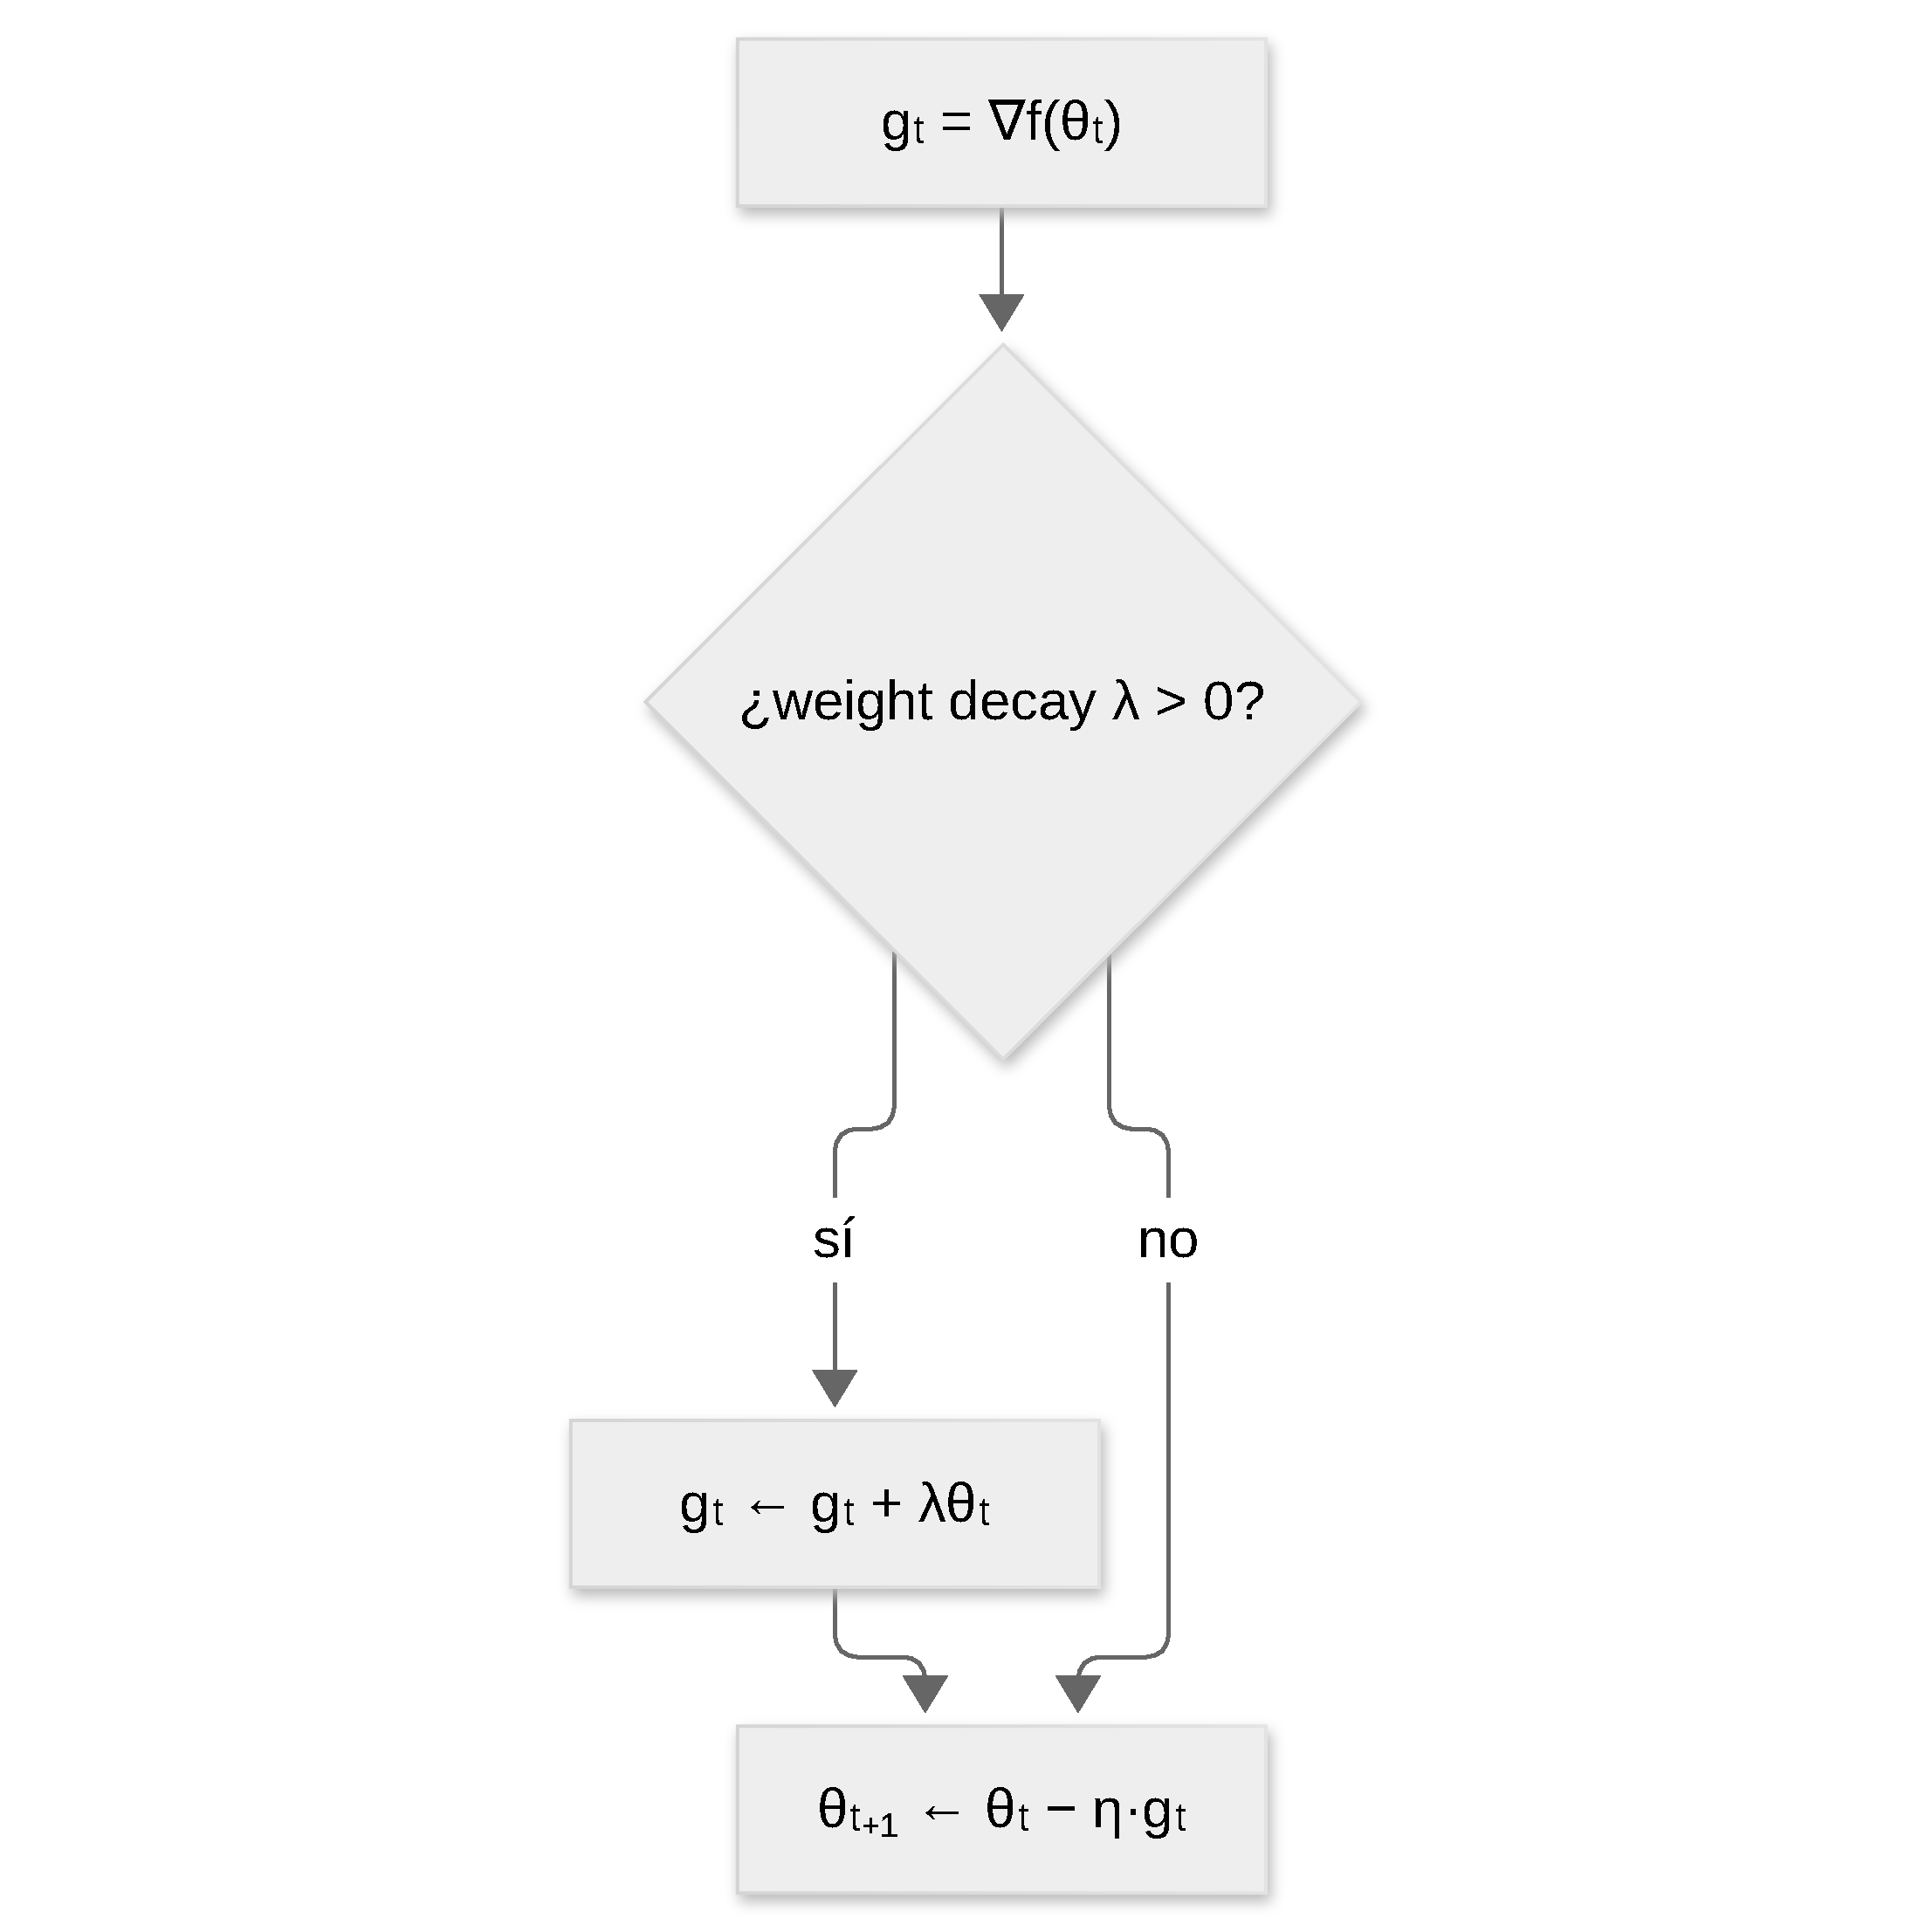
\includegraphics{../paper/figures/optimizers/sgd-es.pdf}}
\caption{Flujo por paso de SGD por mini-lotes: decaimiento L2 opcional y la actualización por gradiente escalado, sin estado del optimizador entre pasos.}
\label{fig:opt-sgd}
\end{figure}
El método de primer orden más simple: actualizar los pesos con el gradiente del mini-lote actual en lugar del lote completo~\citep{hinton_csc321_2012}. En conjuntos de datos redundantes el gradiente del mini-lote es casi tan informativo como el completo, y calcularlo con productos matriz--matriz lo hace mucho más barato que las actualizaciones en línea, especialmente en GPU. En la iteración $t$ con mini-lote $B$:
\begin{align}
g_t &= \frac{1}{|B|} \sum_{i \in B} \nabla_\theta E_i(\theta_t) \\
\theta_{t+1} &= \theta_t - \eta\, g_t
\end{align}
donde $\eta$ es el único hiperparámetro del método. La receta de ajuste de las diapositivas es heurística: reducir la tasa cuando el error oscila o diverge, aumentarla cuando el error baja de forma consistente pero lenta, y bajarla hacia el final del entrenamiento~\citep{hinton_csc321_2012}. El momentum es una extensión separada (párrafo siguiente); esta entrada es deliberadamente la línea base sin estado del catálogo.

\begin{algorithm}[H]
\caption{Descenso de Gradiente Estocástico por Mini-lotes}
\label{alg:sgd}
\begin{algorithmic}[1]
\Require Parámetros iniciales $\theta_0$, tasa de aprendizaje $\eta$, decadencia de peso $\lambda$
\Ensure Parámetros actualizados $\theta_T$
\For{$t = 0, 1, 2, \ldots, T-1$}
    \State Muestrear un mini-lote $B_t$; calcular $g_t \gets \frac{1}{|B_t|}\sum_{i \in B_t}\nabla f_i(\theta_t)$
    \If{decadencia\_de\_peso $> 0$}
        \State $g_t \gets g_t + \lambda \theta_t$ \Comment{Regularización L2}
    \EndIf
    \State Actualizar parámetros: $\theta_{t+1} \gets \theta_t - \eta\, g_t$
\EndFor
\Return $\theta_T$
\end{algorithmic}
\end{algorithm}

\paragraph{Contras.}
\begin{itemize}[leftmargin=*]
\item Una única tasa global no puede adaptarse a curvaturas heterogéneas: el método zigzaguea en valles estrechos y se estanca en direcciones planas.
\item Fuerte dependencia de programaciones de tasa ajustadas a mano; sin adaptividad por parámetro.
\end{itemize}

\paragraph{Ventajas.}
\begin{itemize}[leftmargin=*]
\item Cero estado del optimizador: el piso de memoria del catálogo y el paso más barato.
\item Completamente determinista dado el orden de los lotes; el punto de referencia contra el que se mide cada otra entrada.
\end{itemize}

\paragraph{SGD con Momentum.}
\begin{figure}[H]
\centering
\fitfigure{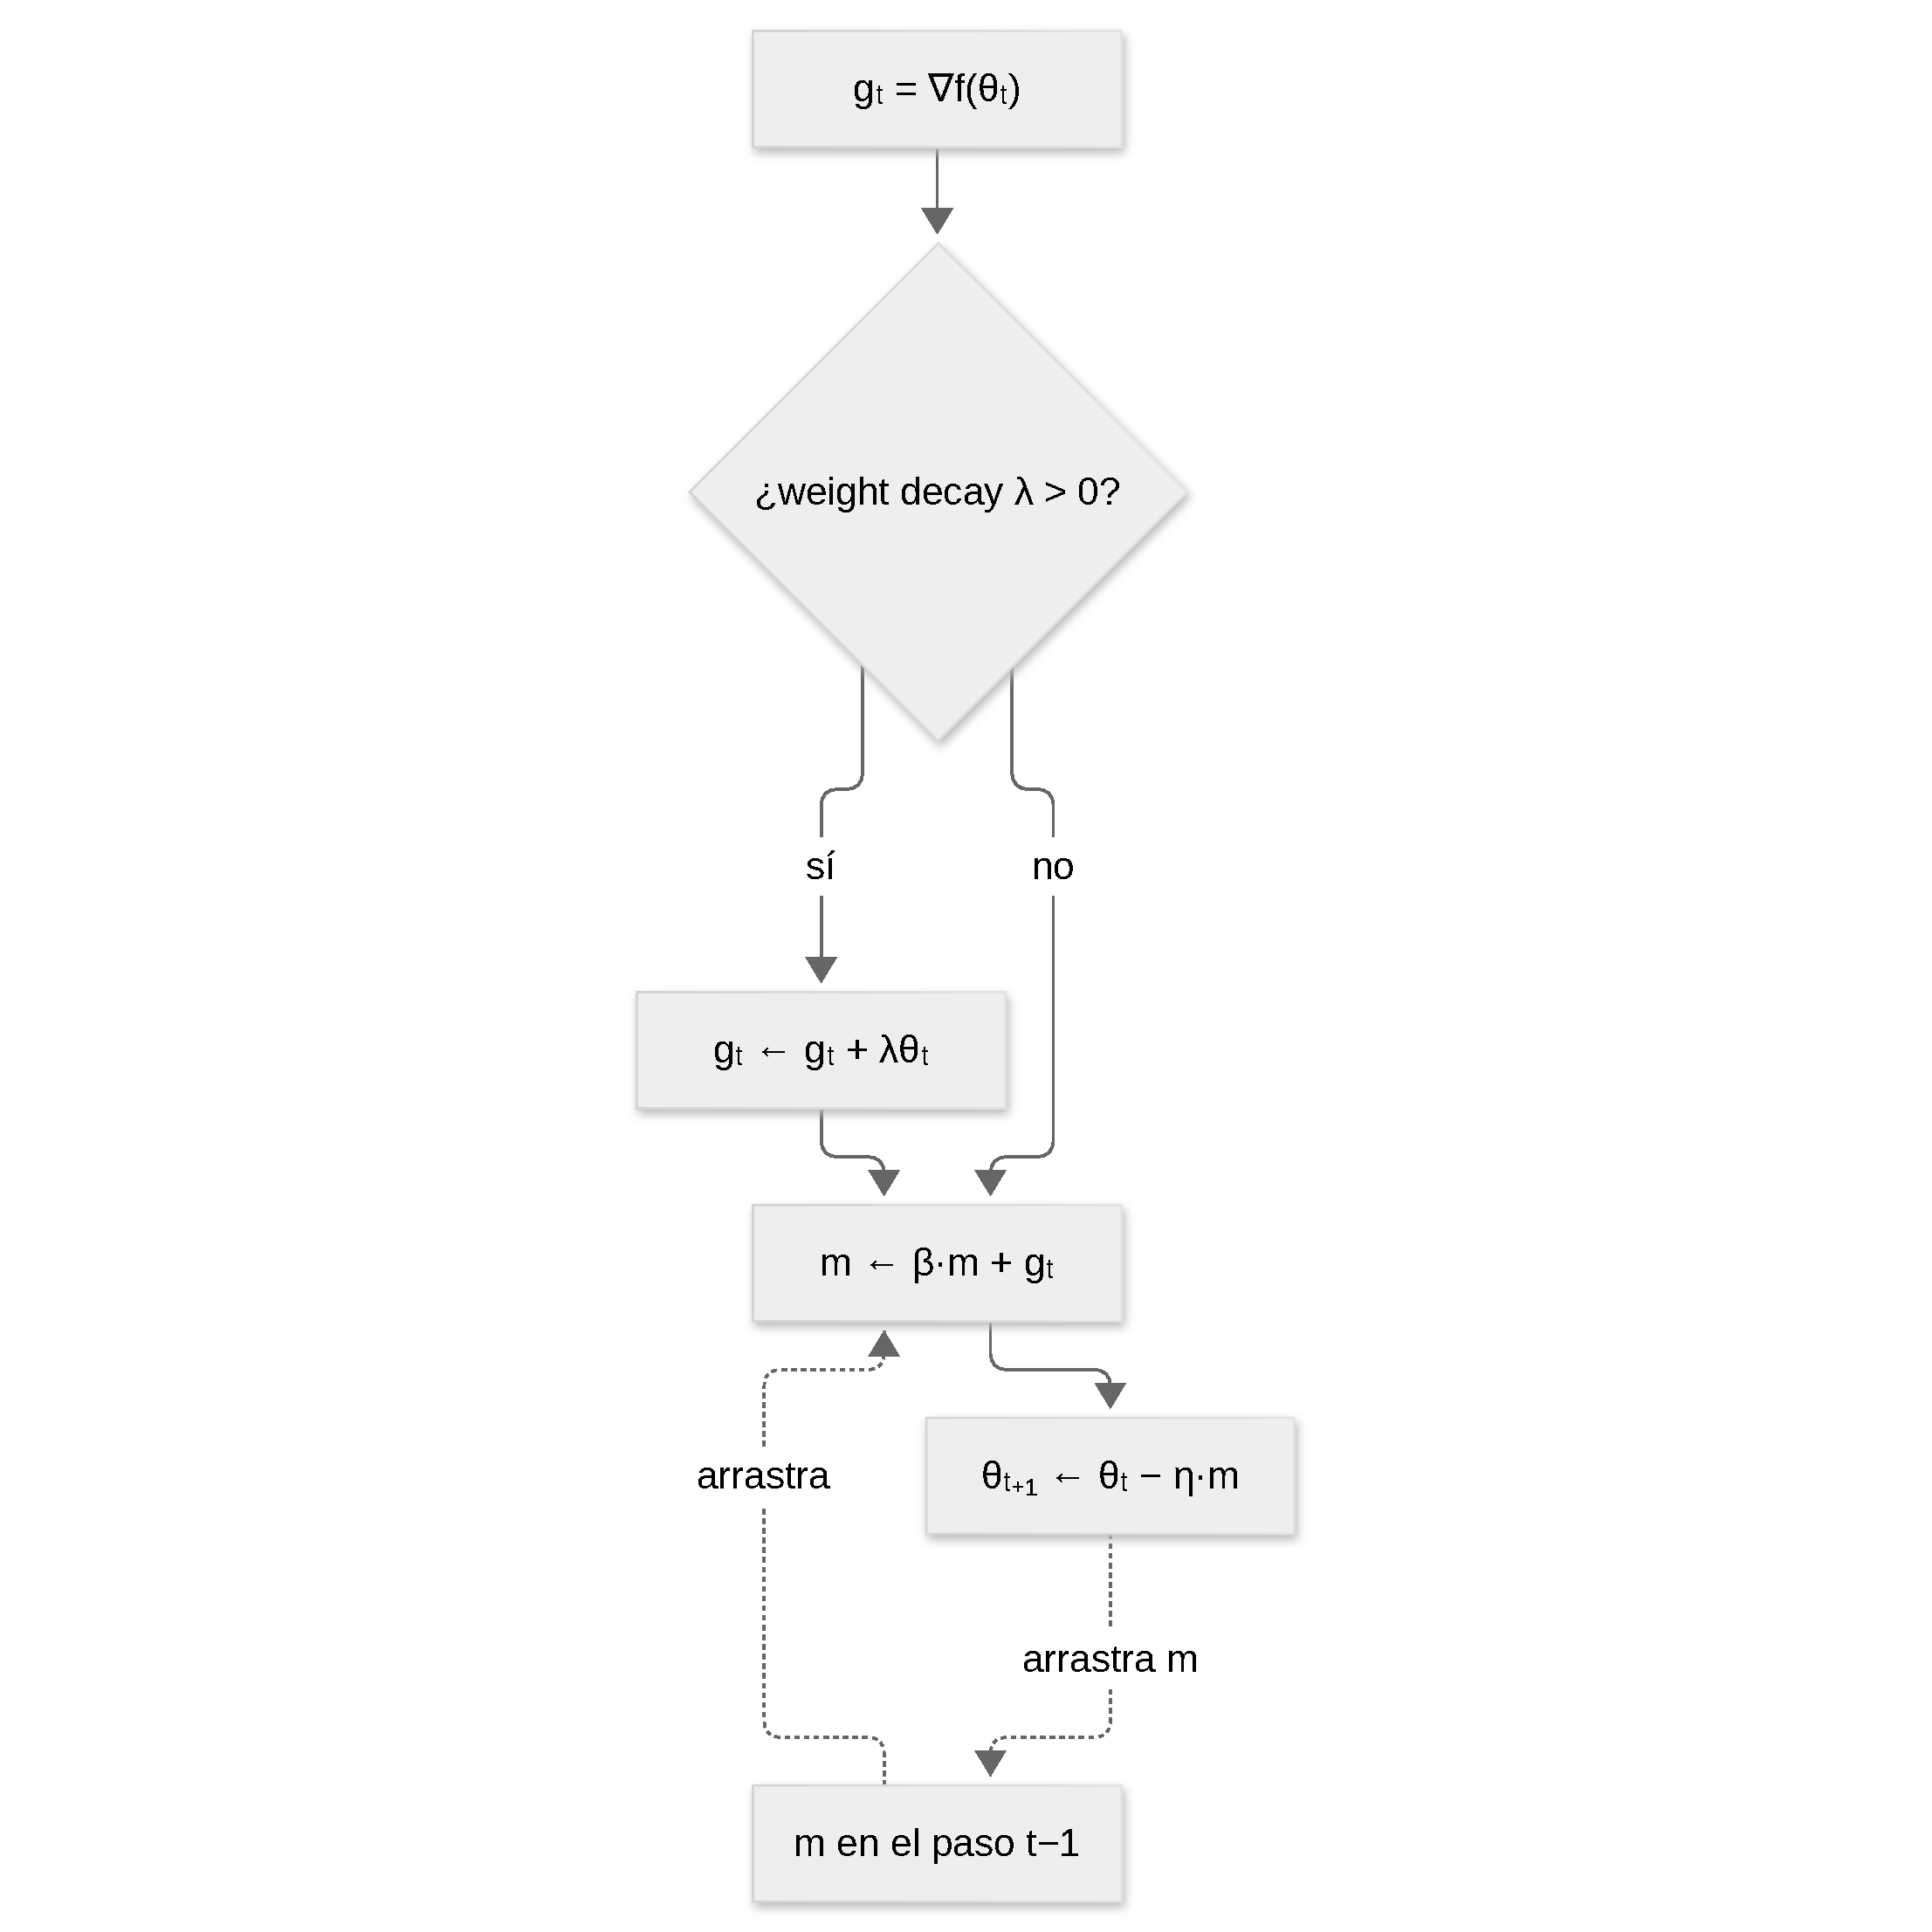
\includegraphics{../paper/figures/optimizers/sgd-momentum-es.pdf}}
\caption{Flujo por paso de SGD con momentum: decaimiento L2 opcional, acumulación exponencial de momentum y actualización de parámetros con paso fijo.}
\label{fig:opt-sgd-momentum}
\end{figure}
La actualización clásica acumula un búfer de momentum y luego aplica una tasa de aprendizaje fija. En cada iteración $t$, el algoritmo mantiene un promedio móvil exponencial $m_t$ de los gradientes pasados:
\begin{align}
m_t &= \beta m_{t-1} + g_t \\
\theta_{t+1} &= \theta_t - \eta m_t
\end{align}
donde $g_t = \nabla f(\theta_t)$, $\beta \in [0.8, 0.99]$ controla la decadencia del momentum y $\eta$ es la tasa de aprendizaje fija. El término de momentum actúa como velocidad: acelera el movimiento en direcciones consistentes mientras amortigua oscilaciones en direcciones variables.

\begin{algorithm}[H]
\caption{SGD con Momentum}
\label{alg:sgd-momentum}
\begin{algorithmic}[1]
\Require Parámetros iniciales $\theta_0$, tasa de aprendizaje $\eta$, coeficiente de momentum $\beta$, decadencia de peso $\lambda$
\Ensure Parámetros actualizados $\theta_T$
\State Inicializar: búfer de momentum $m \gets 0$
\For{$t = 0, 1, 2, \ldots, T-1$}
    \State Calcular gradiente: $g_t \gets \nabla f(\theta_t)$
    \If{decadencia\_de\_peso $> 0$}
        \State $g_t \gets g_t + \lambda \theta_t$ \Comment{Regularización L2}
    \EndIf
    \State Actualizar momentum: $m \gets \beta \cdot m + g_t$
    \State Actualizar parámetros: $\theta_{t+1} \gets \theta_t - \eta \cdot m$
\EndFor
\Return $\theta_T$
\end{algorithmic}
\end{algorithm}

\paragraph{Contras.}
\begin{itemize}[leftmargin=*]
\item Escasa robustez frente a la heterogeneidad de curvatura: una única tasa global no puede adaptarse a todos los grupos de parámetros.
\item Fuerte dependencia de programaciones de tasa de aprendizaje cuidadosamente diseñadas.
\end{itemize}

\paragraph{Ventajas.}
\begin{itemize}[leftmargin=*]
\item Baja sobrecarga de memoria: un único búfer de momentum por parámetro.
\item Fuerte generalización cuando se ajusta cuidadosamente, y una actualización simple de implementar.
\end{itemize}

\paragraph{RMSProp.}
\begin{figure}[H]
\centering
\fitfigure{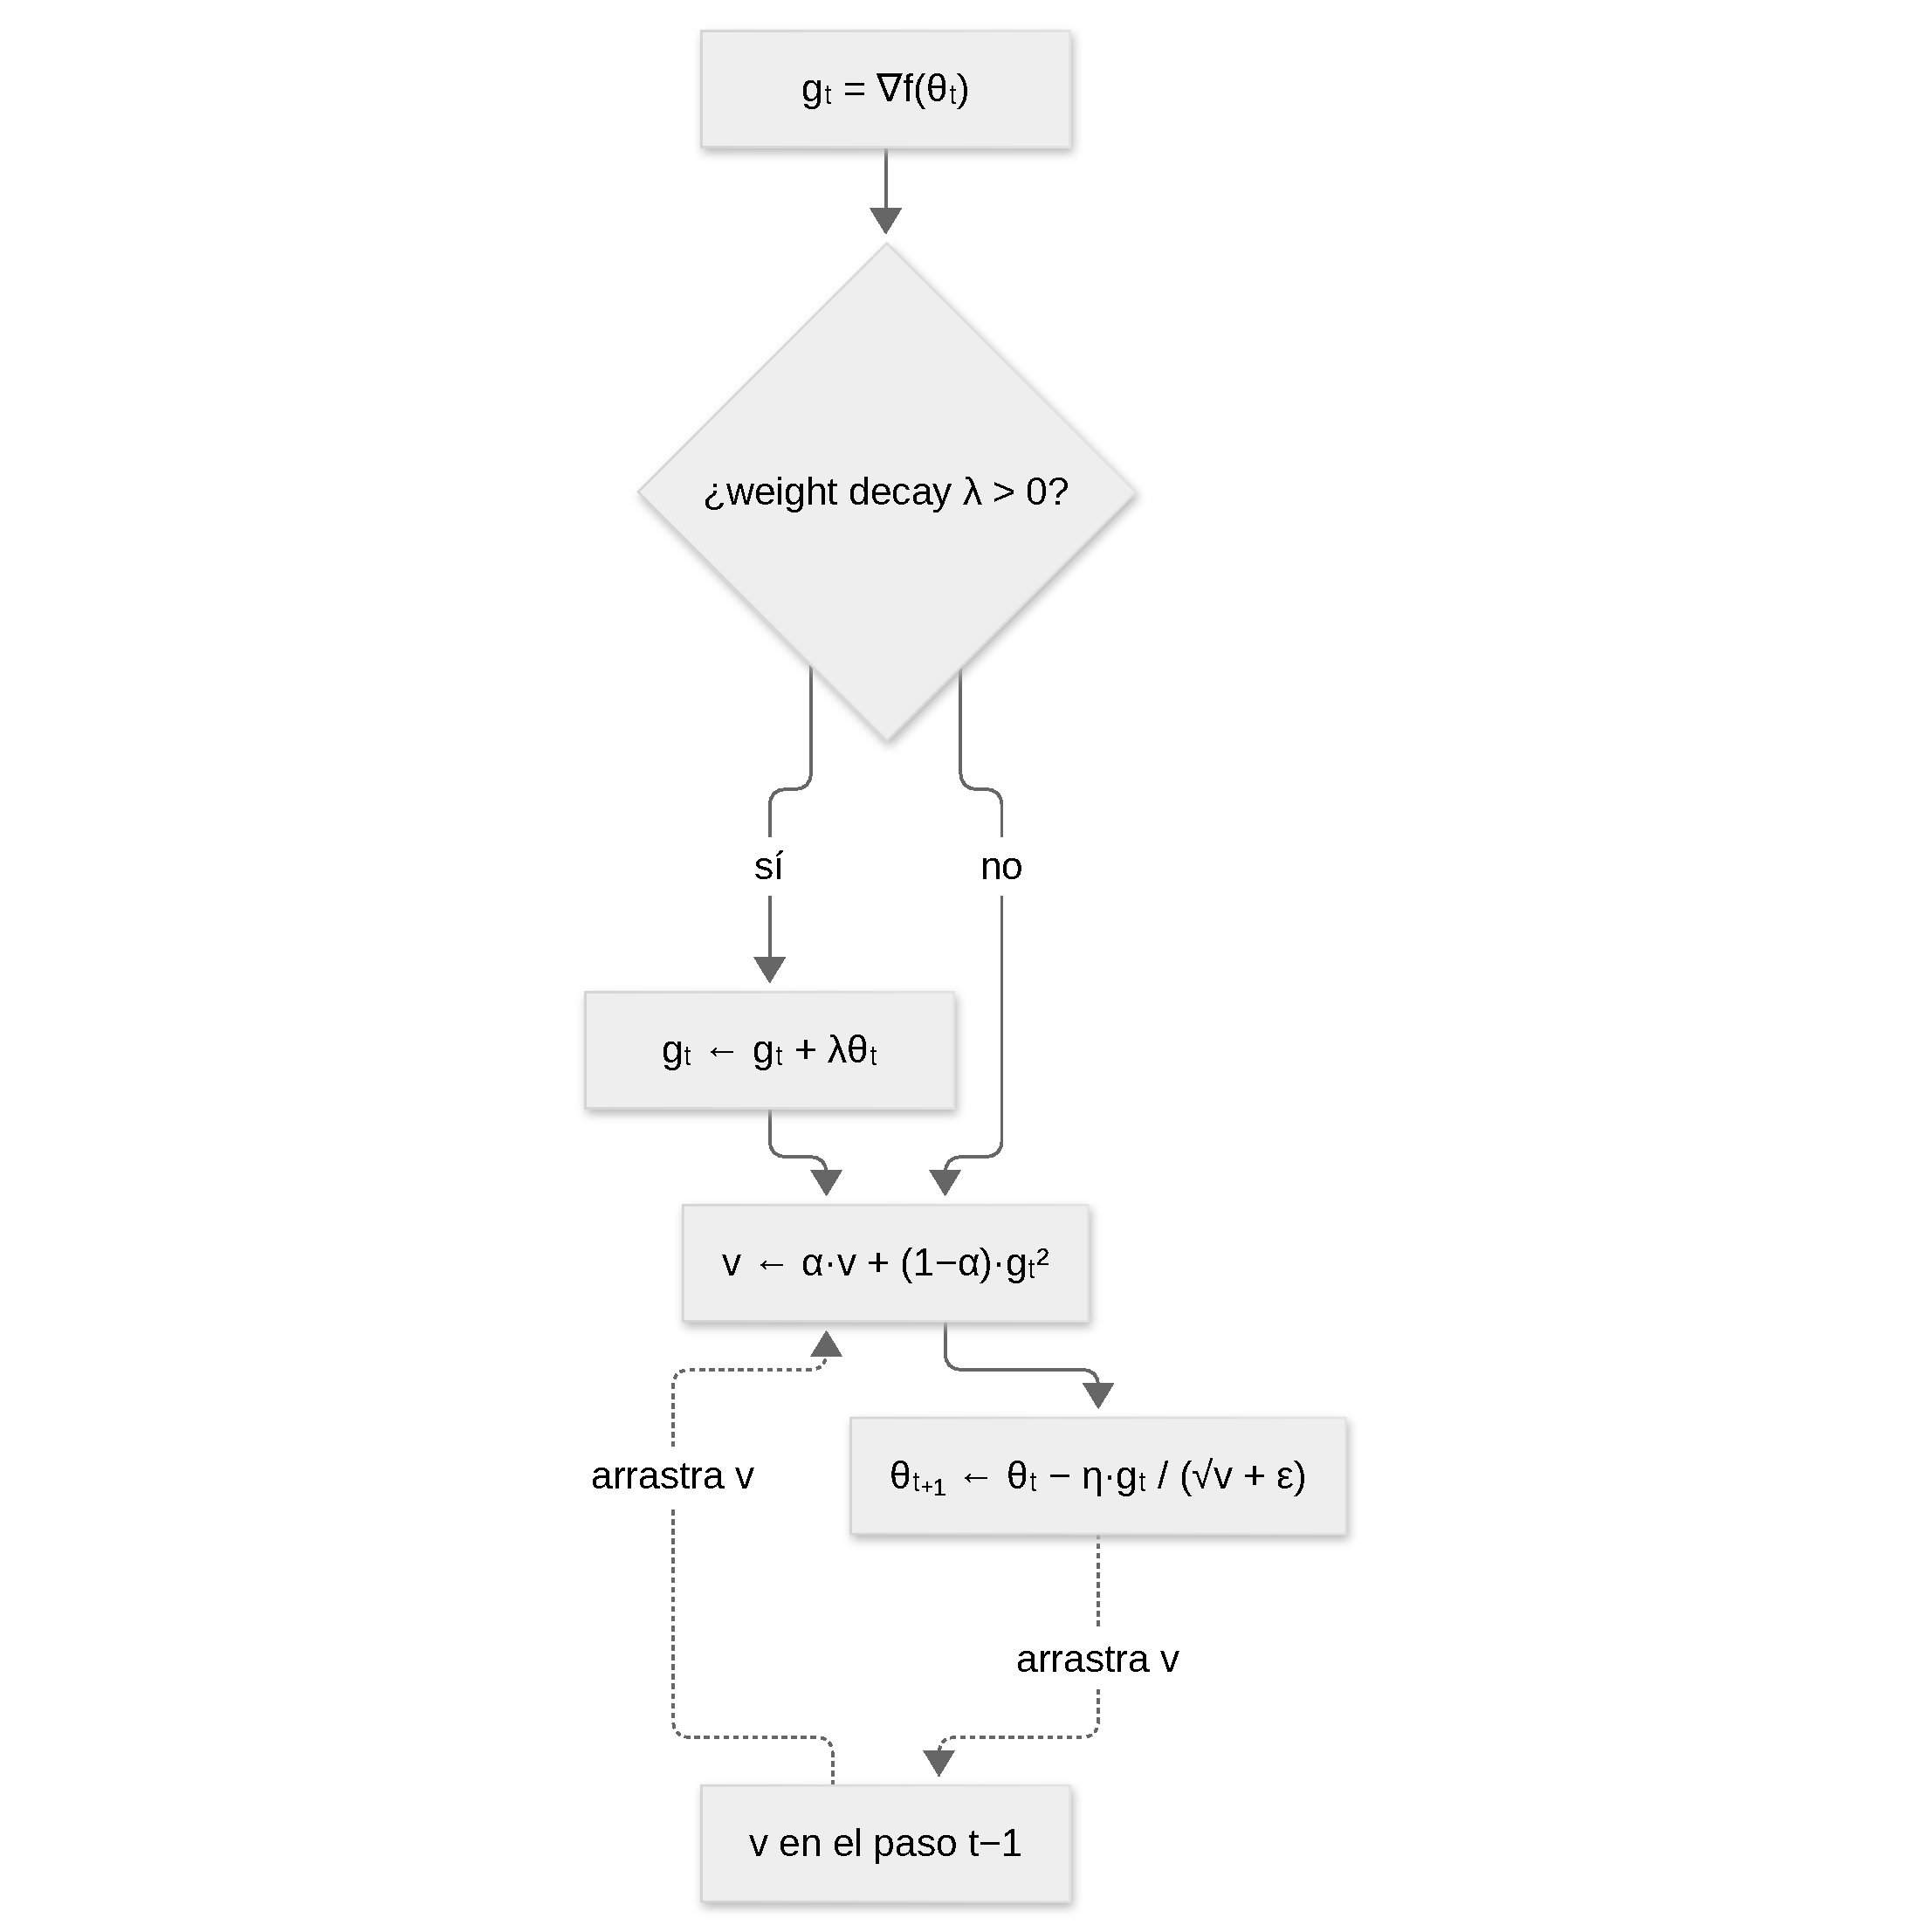
\includegraphics{../paper/figures/optimizers/rmsprop-es.pdf}}
\caption{Flujo por paso de RMSProp: decaimiento L2 opcional, el promedio móvil $v_t$ de gradientes al cuadrado y la división por coordenada por $\sqrt{v_t}$.}
\label{fig:opt-rmsprop}
\end{figure}
RMSProp es la versión segura para mini-lotes de rprop: en lugar de dividir por el tamaño del gradiente actual, se fuerza a que el divisor sea casi idéntico para mini-lotes adyacentes manteniendo un promedio móvil del gradiente al cuadrado por cada peso~\citep{tieleman_hinton2012}:
\begin{align}
v_t &= 0.9\, v_{t-1} + 0.1\, g_t^2 \\
\theta_{t+1} &= \theta_t - \eta\, \frac{g_t}{\sqrt{v_t} + \epsilon}
\end{align}
donde $g_t = \partial E/\partial w(t)$, la división $0.9/0.1$ es el decaimiento exponencial de las diapositivas (expuesto como el hiperparámetro \texttt{alpha}) y $\epsilon$ es una guarda numérica añadida por la implementación (las diapositivas no definen ninguna). El método original no incluye corrección de sesgo ni primer momento~\citep{tieleman_hinton2012}; combinarlo con momentum queda explícitamente abierto en las diapositivas (``el momentum no ayuda tanto como normalmente''). El promedio móvil es el único búfer de estado y el predecesor directo de la familia adaptativa: la idea diagonal de AdaGrad~\citep{duchi_adagrad_2011} hecha segura para mini-lotes y luego extendida en Adam.

\begin{algorithm}[H]
\caption{RMSProp}
\label{alg:rmsprop}
\begin{algorithmic}[1]
\Require Parámetros iniciales $\theta_0$, tasa de aprendizaje $\eta$, decaimiento $\alpha = 0.9$, épsilon $\epsilon$, decadencia de peso $\lambda$
\Ensure Parámetros actualizados $\theta_T$
\State Inicializar: promedio móvil $v \gets 0$
\For{$t = 0, 1, 2, \ldots, T-1$}
    \State Calcular gradiente: $g_t \gets \nabla f(\theta_t)$
    \If{decadencia\_de\_peso $> 0$}
        \State $g_t \gets g_t + \lambda \theta_t$ \Comment{Regularización L2}
    \EndIf
    \State Actualizar promedio móvil: $v \gets \alpha v + (1-\alpha) g_t^2$
    \State Actualizar parámetros: $\theta_{t+1} \gets \theta_t - \eta\, g_t / (\sqrt{v} + \epsilon)$
\EndFor
\Return $\theta_T$
\end{algorithmic}
\end{algorithm}

\paragraph{Contras.}
\begin{itemize}[leftmargin=*]
\item Sin corrección de sesgo: el divisor está inflado al inicio del entrenamiento, cuando $v_t$ todavía es una estimación pobre.
\item Sigue siendo sensible al ajuste (tasa, decaimiento, épsilon) y fue en gran medida superado por Adam para transformers.
\end{itemize}

\paragraph{Ventajas.}
\begin{itemize}[leftmargin=*]
\item Un búfer por parámetro y un paso $\mathcal{O}(n)$: el método adaptativo más barato del catálogo.
\item El escalado por coordenada mantiene el paso robusto frente a magnitudes de gradiente heterogéneas entre capas.
\end{itemize}

\paragraph{Adam y AdamW.}
\begin{figure}[H]
\centering
\fitfigure{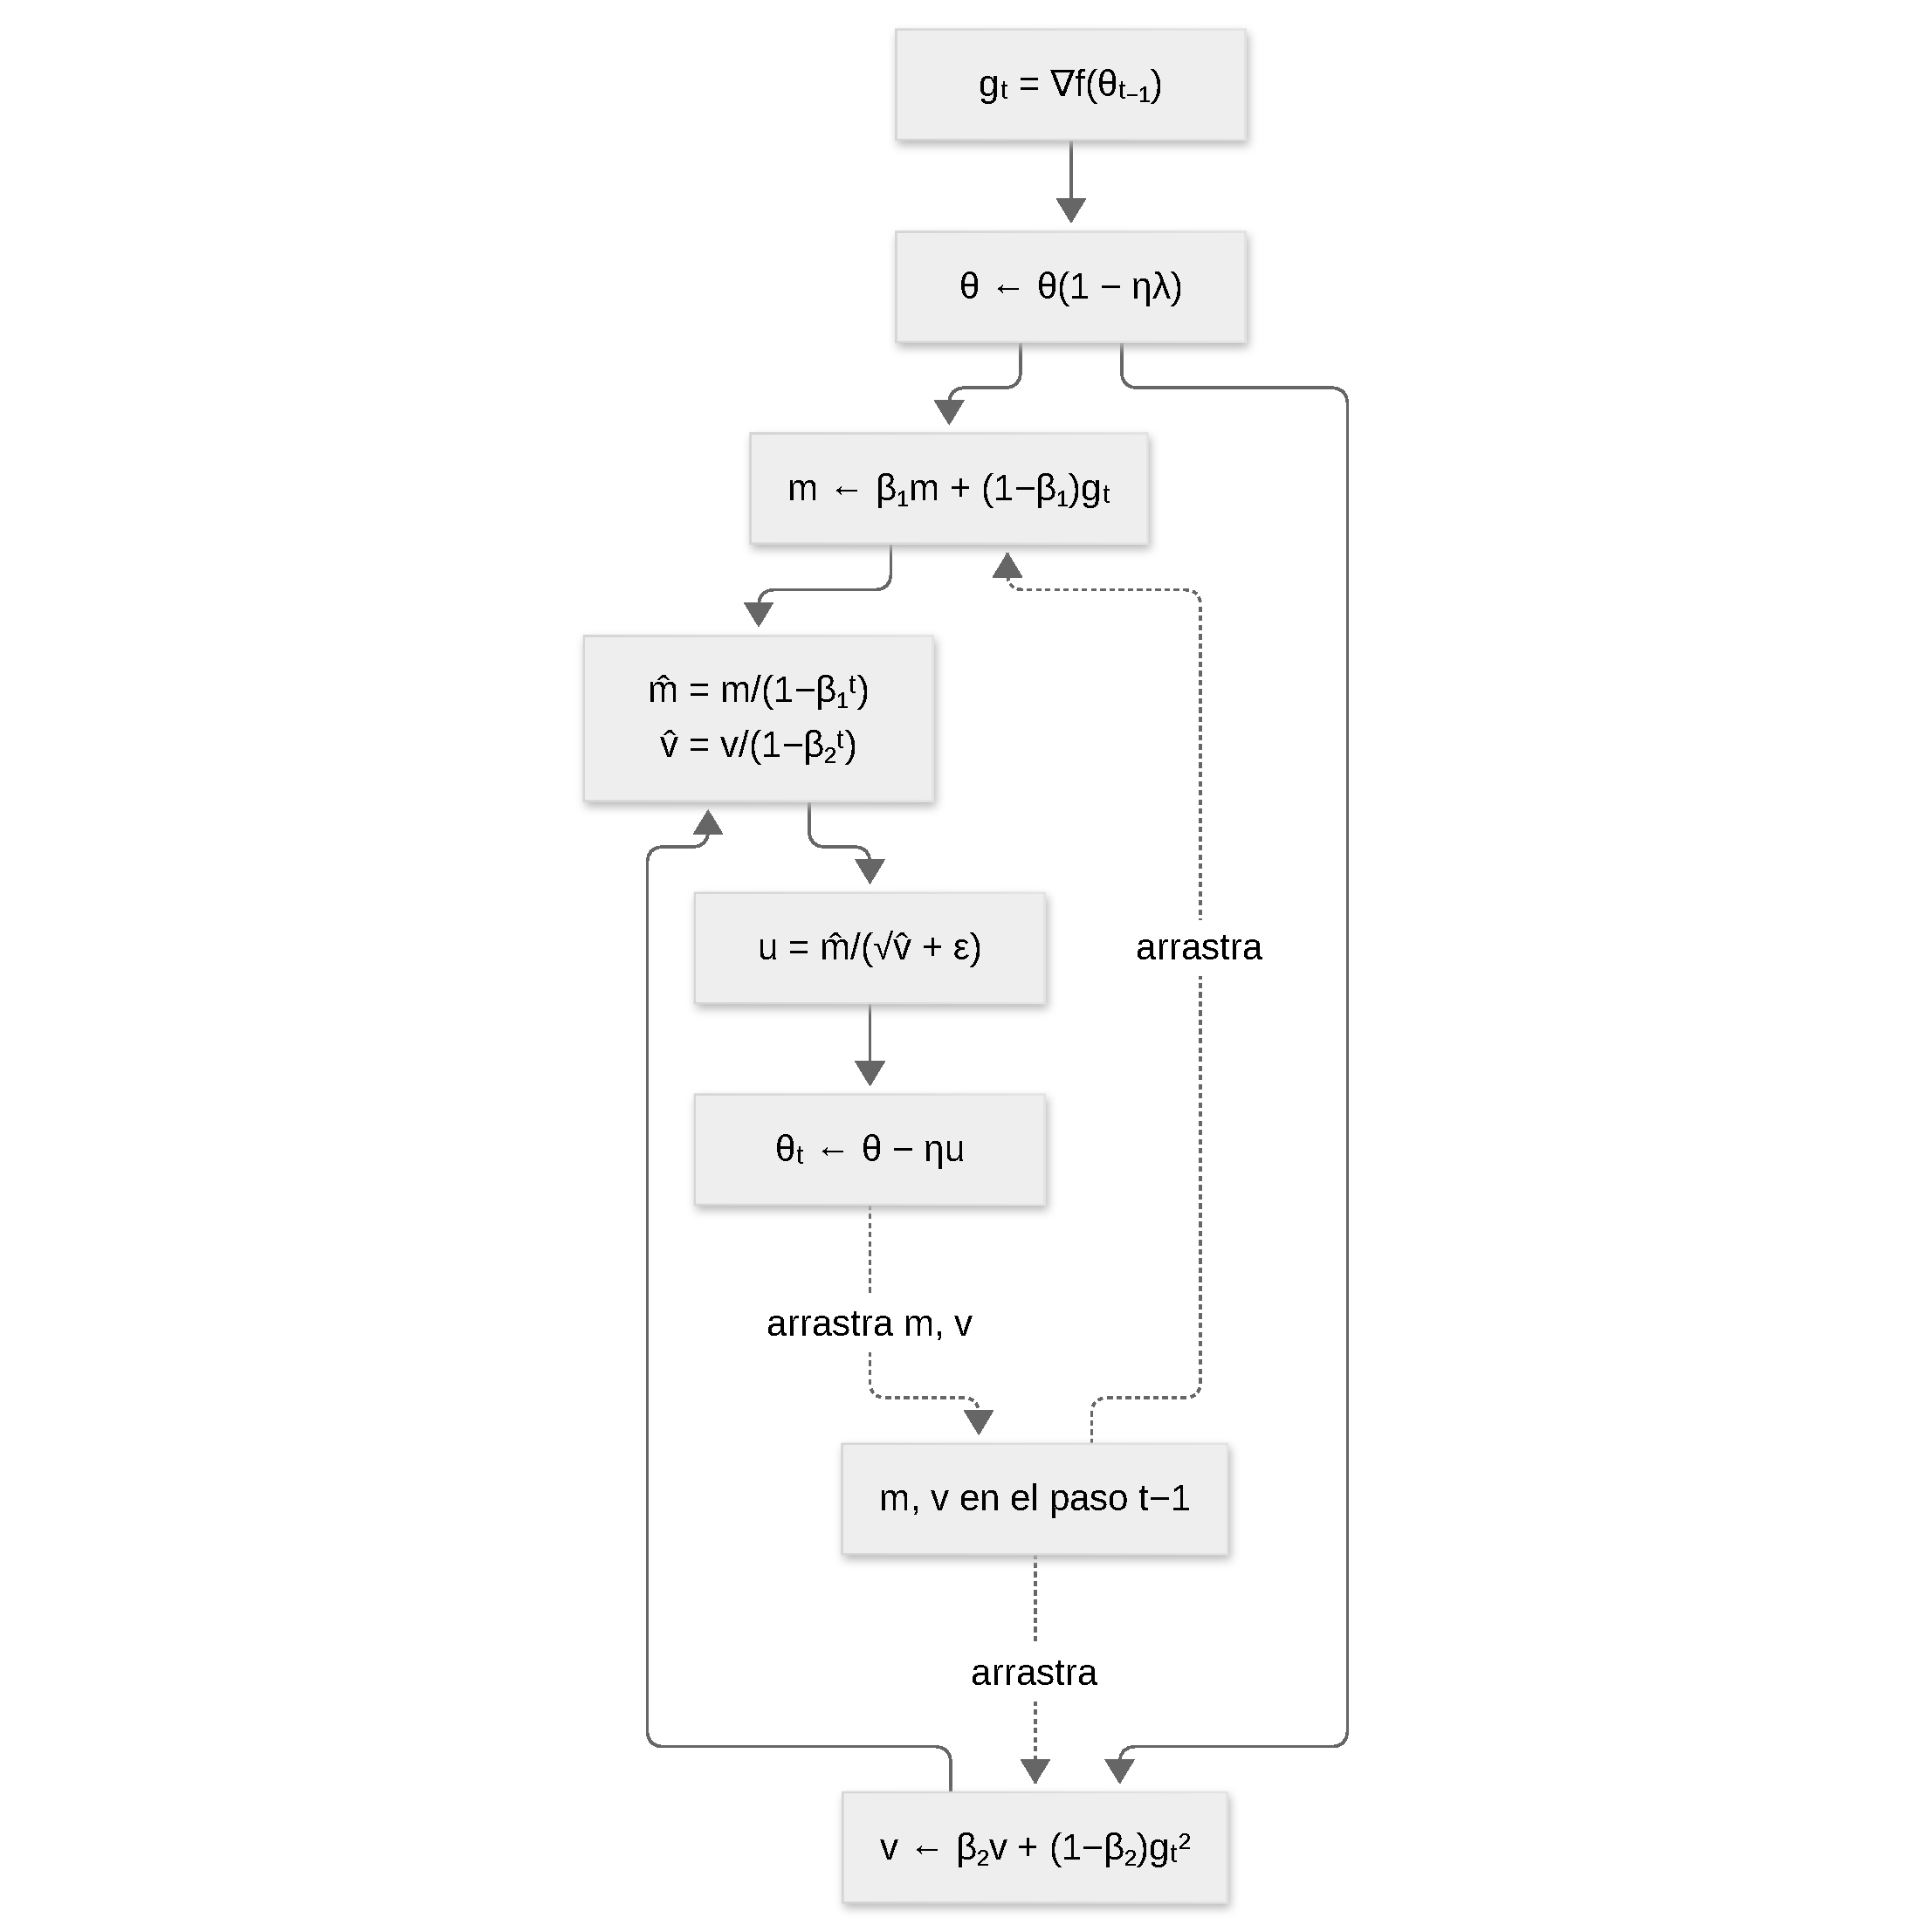
\includegraphics{../paper/figures/optimizers/adamw-es.pdf}}
\caption{Flujo por paso de AdamW: decaimiento de pesos desacoplado, EMAs de primer y segundo momento, corrección de sesgo y actualización adaptativa elemento a elemento.}
\label{fig:opt-adamw}
\end{figure}
Adam rastrea promedios móviles exponenciales tanto del primer momento (media) como del segundo momento (varianza no centrada) para lograr tasas de aprendizaje adaptativas elemento a elemento. La regla de actualización es:
\begin{align}
m_t &= \beta_1 m_{t-1} + (1-\beta_1) g_t \\
v_t &= \beta_2 v_{t-1} + (1-\beta_2) g_t^2 \\
\hat{m}_t &= \frac{m_t}{1-\beta_1^t}, \quad \hat{v}_t = \frac{v_t}{1-\beta_2^t} \quad \text{(corrección de sesgo)} \\
\theta_{t+1} &= \theta_t - \eta \left(\frac{\hat{m}_t}{\sqrt{\hat{v}_t}+\epsilon}\right)
\end{align}
AdamW introduce una modificación crucial: la decadencia de peso se aplica directamente a los parámetros (desacoplada de los gradientes): $\theta_t \gets \theta_t(1-\eta\lambda)$ en lugar de añadir $\lambda\theta_t$ al gradiente. Este desacoplamiento evita que el escalado adaptativo interfiera con la fuerza de la regularización.

\begin{algorithm}[H]
\caption{AdamW (Adam con Decadencia de Peso Desacoplada)}
\label{alg:adamw}
\begin{algorithmic}[1]
\Require Parámetros iniciales $\theta_0$, tasa de aprendizaje $\eta$, tasas de decadencia exponencial $\beta_1, \beta_2 \in [0,1)$
\Require Constante de momentum $\epsilon$, decadencia de peso $\lambda$
\Ensure Parámetros actualizados $\theta_T$
\State Inicializar: primer momento $m \gets 0$, segundo momento $v \gets 0$, contador de pasos $t \gets 0$
\For{$t = 1, 2, \ldots, T$}
    \State Calcular gradiente: $g_t \gets \nabla f(\theta_{t-1})$
    \State Decadencia de peso (desacoplada): $\theta_{t-1} \gets \theta_{t-1}(1 - \eta\lambda)$
    \State Actualizar momentos: $m \gets \beta_1 m + (1-\beta_1) g_t$
    \State $v \gets \beta_2 v + (1-\beta_2) g_t^2$
    \State Corrección de sesgo: $\hat{m} \gets m / (1 - \beta_1^t)$, $\hat{v} \gets v / (1 - \beta_2^t)$
    \State Actualizar parámetros: $\theta_t \gets \theta_{t-1} - \eta (\hat{m} / (\sqrt{\hat{v}} + \epsilon))$
\EndFor
\Return $\theta_T$
\end{algorithmic}
\end{algorithm}

\paragraph{Contras.}
\begin{itemize}[leftmargin=*]
\item Almacena tensores de primer y segundo momento para cada parámetro, duplicando la memoria del estado del optimizador respecto a SGD.
\item El escalado adaptativo elemento a elemento puede interferir con la regularización si el decaimiento de pesos no se desacopla.
\end{itemize}

\paragraph{Ventajas.}
\begin{itemize}[leftmargin=*]
\item Línea base práctica para el ajuste fino de transformadores: convergencia rápida y tolerancia a la variación de hiperparámetros.
\item El decaimiento de pesos desacoplado mantiene la fuerza de la regularización independiente del escalado adaptativo.
\end{itemize}

\paragraph{RAdam (Adam Rectificado).}
\begin{figure}[H]
\centering
\fitfigure{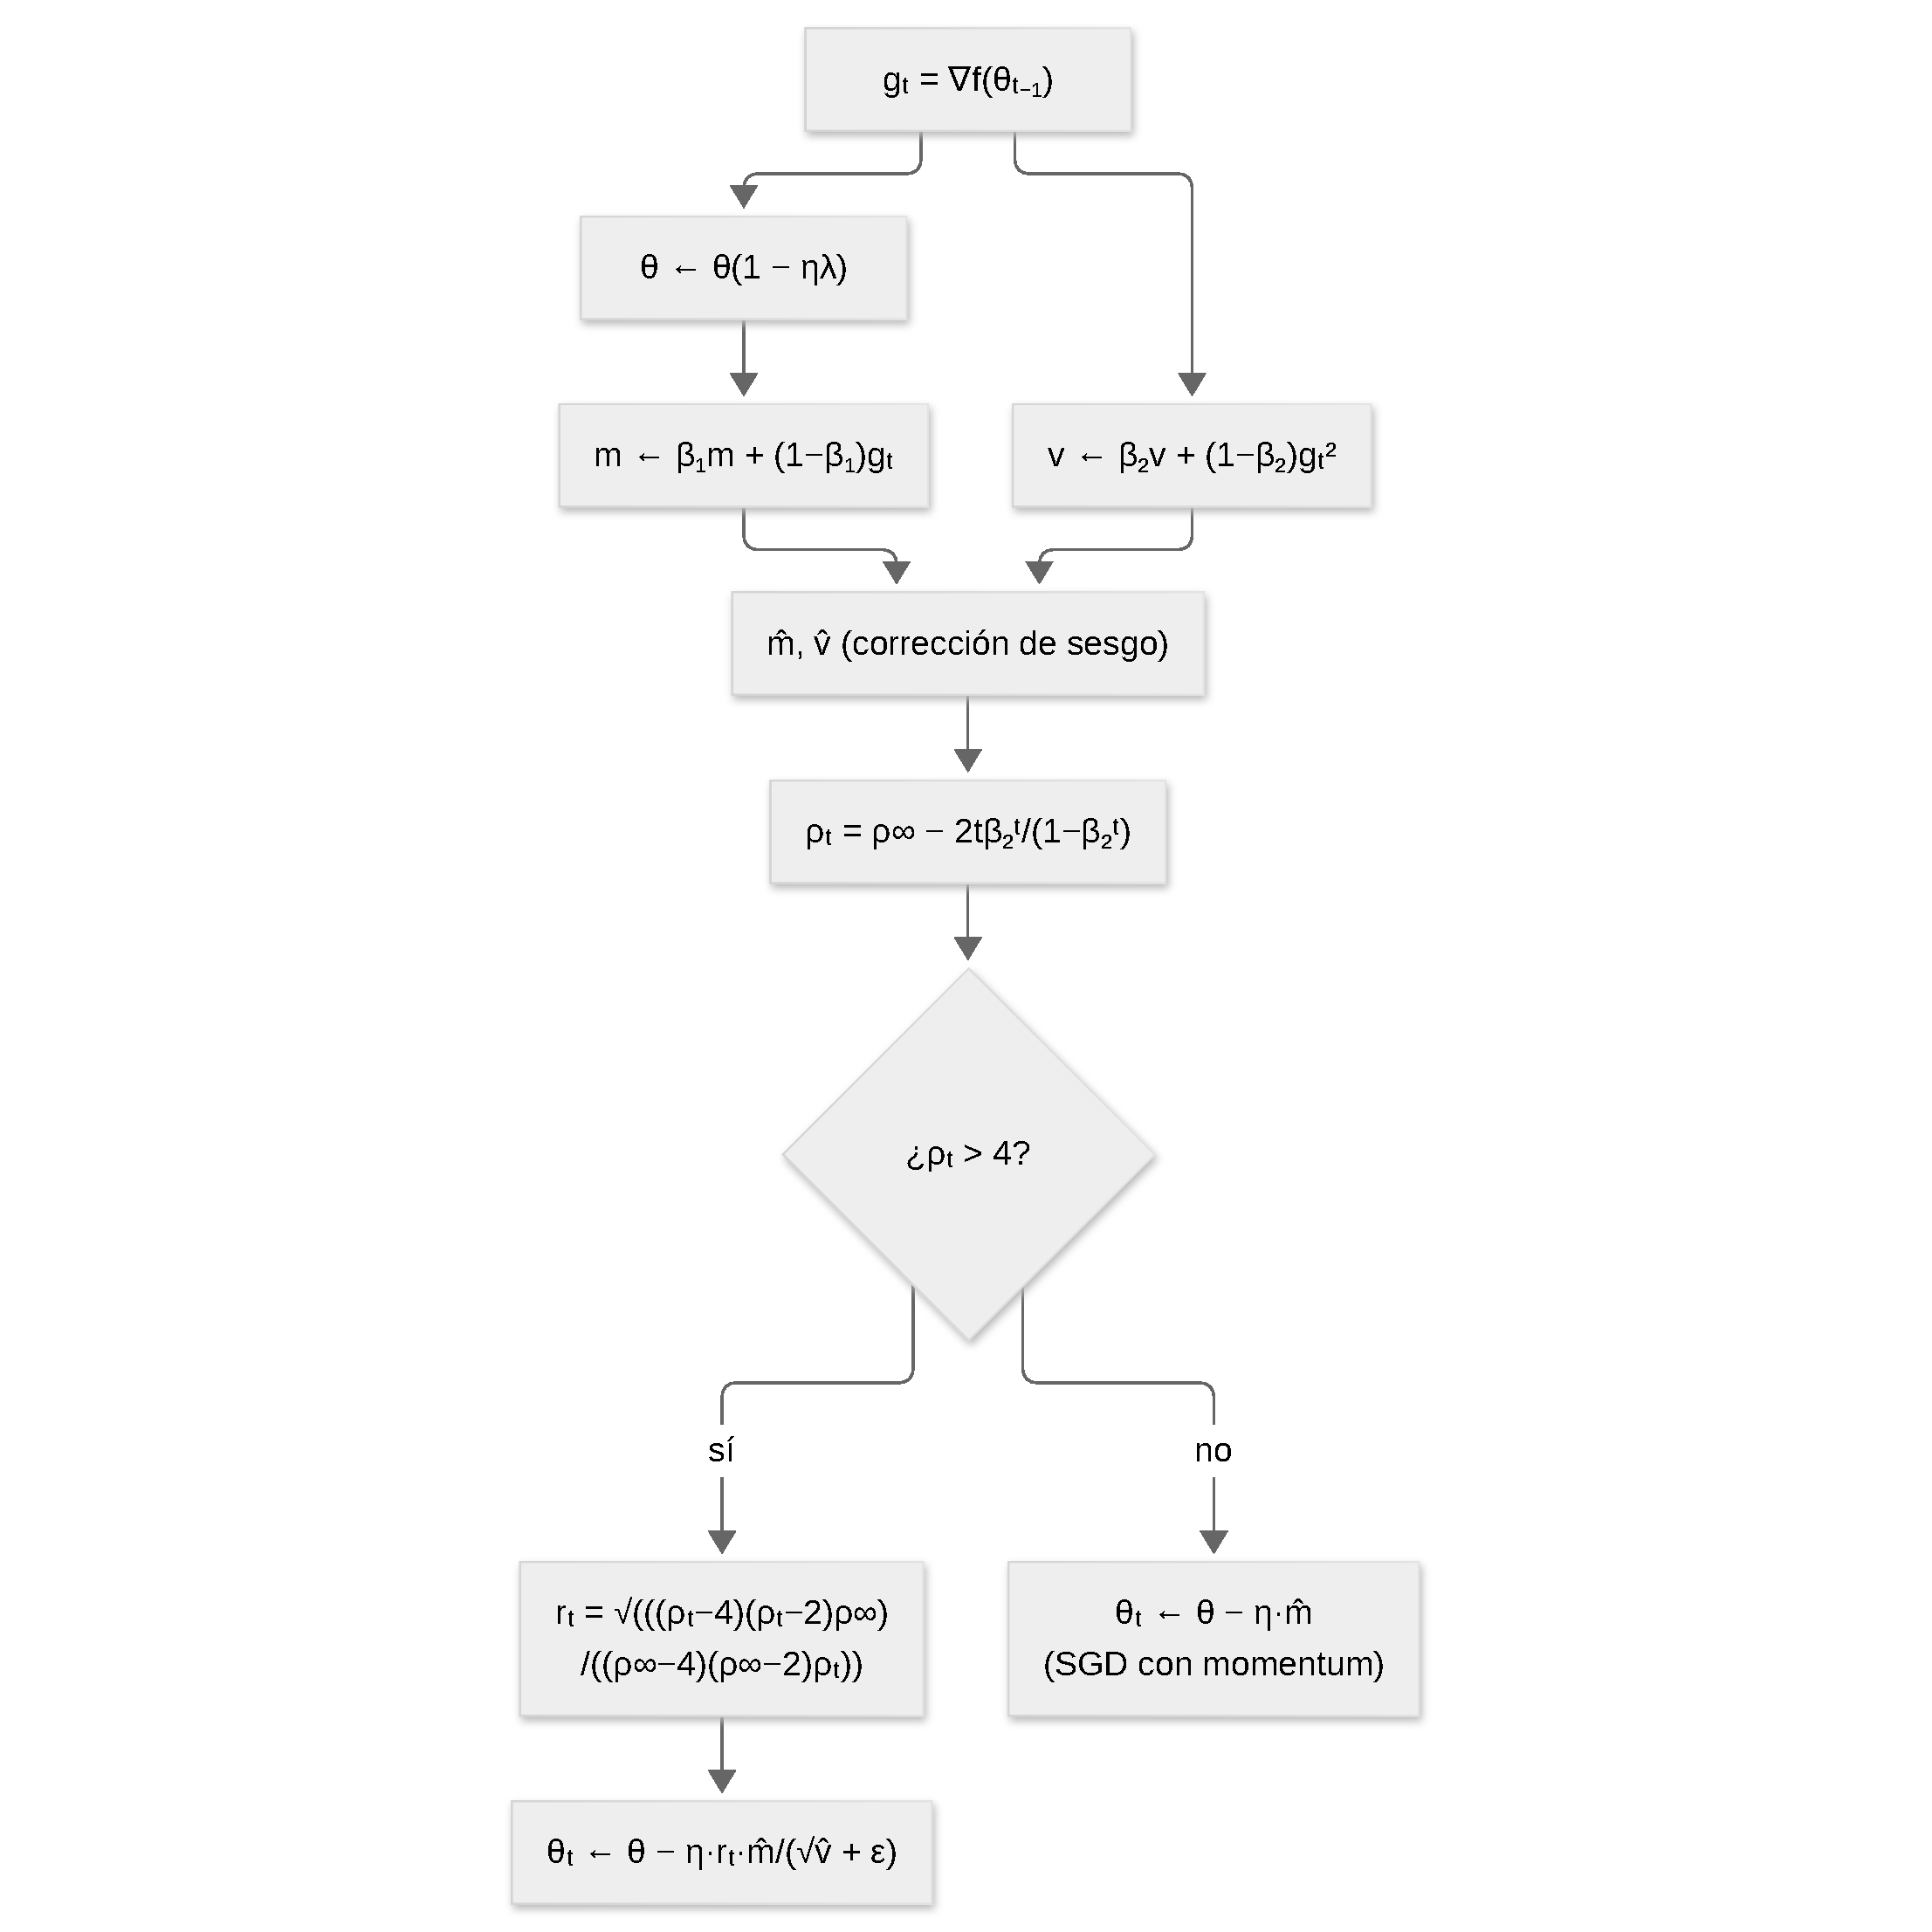
\includegraphics{../paper/figures/optimizers/radam-es.pdf}}
\caption{Flujo por paso de RAdam: rectificación por ventana SMA con retroceso a SGD con momentum en los primeros pasos.}
\label{fig:opt-radam}
\end{figure}
RAdam aborda la inestabilidad de Adam en el entrenamiento temprano rectificando dinámicamente la tasa de aprendizaje adaptativa. La observación clave es que el segundo momento $v_t$ tiene una varianza muy alta en los primeros pasos, causando un escalado adaptativo poco fiable. RAdam calcula la longitud efectiva de la ventana de promedio móvil simple (SMA):
\[\rho_t = \rho_{\infty} - \frac{2t\beta_2^t}{1-\beta_2^t}, \quad \text{donde} \quad \rho_{\infty} = \frac{2}{1-\beta_2}-1\]
Cuando $\rho_t > 4$ (suficientes muestras para la estimación de varianza), RAdam aplica el escalado adaptativo con un término de rectificación:
\[r_t = \sqrt{\frac{(\rho_t-4)(\rho_t-2)\rho_{\infty}}{(\rho_{\infty}-4)(\rho_{\infty}-2)\rho_t}}, \quad \theta_{t+1} = \theta_t - \eta r_t \frac{\hat{m}_t}{\sqrt{\hat{v}_t}+\epsilon}\]
Cuando $\rho_t \leq 4$, RAdam retrocede a SGD con momentum: $\theta_{t+1} = \theta_t - \eta\hat{m}_t$.

\begin{algorithm}[H]
\caption{RAdam (Adam Rectificado)}
\label{alg:radam}
\begin{algorithmic}[1]
\Require Parámetros iniciales $\theta_0$, tasa de aprendizaje $\eta$, $\beta_1, \beta_2$, decadencia de peso $\lambda$
\Ensure Parámetros actualizados $\theta_T$
\State Inicializar: $m \gets 0$, $v \gets 0$, $t \gets 0$
\State Calcular: $\rho_\infty \gets 2/(1-\beta_2) - 1$
\For{$t = 1, 2, \ldots, T$}
    \State $g_t \gets \nabla f(\theta_{t-1})$
    \If{decadencia\_de\_peso $> 0$}
        \State $\theta_{t-1} \gets \theta_{t-1}(1 - \eta\lambda)$
    \EndIf
    \State $m \gets \beta_1 m + (1-\beta_1) g_t$
    \State $v \gets \beta_2 v + (1-\beta_2) g_t^2$
    \State $\hat{m} \gets m/(1-\beta_1^t)$, $\hat{v} \gets v/(1-\beta_2^t)$
    \State $\rho_t \gets \rho_\infty - 2t \beta_2^t / (1 - \beta_2^t)$
    \If{$\rho_t > 4$}
        \State $r_t \gets \sqrt{((\rho_t-4)(\rho_t-2)\rho_\infty) / ((\rho_\infty-4)(\rho_\infty-2)\rho_t)}$
        \State $\theta_t \gets \theta_{t-1} - \eta r_t \hat{m} / (\sqrt{\hat{v}} + \epsilon)$
    \Else
        \State $\theta_t \gets \theta_{t-1} - \eta \hat{m}$ \Comment{SGD con momentum}
    \EndIf
\EndFor
\Return $\theta_T$
\end{algorithmic}
\end{algorithm}

\paragraph{Contras.}
\begin{itemize}[leftmargin=*]
\item Añade contabilidad de rectificación sobre el estado de momentos de Adam.
\item El beneficio se reduce cuando ya se usa una programación de calentamiento bien ajustada.
\end{itemize}

\paragraph{Ventajas.}
\begin{itemize}[leftmargin=*]
\item Elimina la necesidad de calentamiento manual al rectificar la tasa adaptativa.
\item Retrocede con elegancia a SGD con momentum mientras las estimaciones de varianza no son fiables, mejorando la robustez.
\end{itemize}


\paragraph{LaProp.}
LaProp ataca un acoplamiento innecesario en Adam en lugar de un nuevo
precondicionador~\citep{ziyin_laprop_2021}. Escribiendo la familia adaptativa
como $\theta_{t+1} = \theta_t - \lambda_t G_t \nabla\ell(\theta_t) + \mu_t K_t(\theta_t - \theta_{t-1})$,
el momentum en el espacio de parámetros de Adam queda multiplicado por
$K_t = H_t^{-1}H_{t-1}$, es decir, el movimiento previo se reescala con el
precondicionador actual. Un único gradiente patológicamente grande---ruido, un
lote fuera de distribución o una explosión---puede por tanto borrar el momentum
acumulado. LaProp simplemente fija $K_t = I$ y, en su lugar, acumula el momentum
del gradiente \emph{precondicionado}:
\begin{align}
n_t &= \nu n_{t-1} + (1-\nu) g_t^2 \\
m_t &= \mu m_{t-1} + (1-\mu)\,\frac{g_t}{\sqrt{n_t/(1-\nu^t)} + \epsilon} \\
\theta_{t+1} &= \theta_t - \lambda\,\frac{m_t}{1-\mu^t}
\end{align}
con $g_t = \nabla\ell(\theta_t)$ y $0 \le \mu, \nu < 1$. El segundo momento
$n_t$ es la varianza no centrada de Adam; el primer momento $m_t$ promedia la
dirección ya normalizada, de modo que el momentum en el espacio de parámetros
permanece aditivo como en SGD. La influencia de cualquier gradiente individual
sobre el momentum acumulado está acotada por $(1-\mu)/\sqrt{1-\nu}$. LaProp
tiene exactamente el estado (dos búferes), el costo por paso y el número de
hiperparámetros de Adam, y los ajustes de Adam se transfieren sin cambios;
$\nu \to 0$ recupera los métodos de gradiente con signo y $\mu = 0$ recupera
RMSProp con corrección de sesgo (el artículo lo describe como RMSProp con
momentum más ambos factores de corrección).

\begin{algorithm}[H]
\caption{LaProp}
\label{alg:laprop}
\begin{algorithmic}[1]
\Require Parámetros iniciales $\theta_1$, tasa de aprendizaje $\{\lambda_t\}_{t=1}^T$, parámetros de decaimiento $0 \le \mu, \nu < 1$
\Require Épsilon $\epsilon \ll 1$, decadencia de peso $\lambda_{\mathrm{wd}}$
\Ensure Parámetros actualizados $\theta_T$
\State Inicializar: primer momento $m_0 \gets 0$, segundo momento $n_0 \gets 0$
\For{$t = 1, 2, \ldots, T$}
    \State $g_t \gets \nabla_\theta \ell(\theta_t)$
    \If{decadencia\_de\_peso $> 0$}
        \State $g_t \gets g_t + \lambda_{\mathrm{wd}} \theta_t$ \Comment{Regularización L2}
    \EndIf
    \State $n_t \gets \nu n_{t-1} + (1-\nu) g_t^2$
    \State $m_t \gets \mu m_{t-1} + (1-\mu) g_t / (\sqrt{n_t/(1-\nu^t)} + \epsilon)$
    \State $\theta_{t+1} \gets \theta_t - \lambda_t\, m_t / (1-\mu^t)$
\EndFor
\Return $\theta_T$
\end{algorithmic}
\end{algorithm}

\paragraph{Contras.}
\begin{itemize}[leftmargin=*]
\item No domina a Adam en todas las tareas; sus mejoras se concentran en regímenes de optimización ruidosos o inestables.
\item Acopla el decaimiento del momentum a la escala precondicionada, por lo que el tamaño de paso efectivo al inicio difiere del de Adam hasta que se estabiliza la corrección de sesgo.
\end{itemize}

\paragraph{Ventajas.}
\begin{itemize}[leftmargin=*]
\item Memoria ($m$, $v$), costo por paso y número de hiperparámetros idénticos a Adam; los ajustes existentes de Adam se transfieren directamente.
\item Mantiene aditivo el momentum en el espacio de parámetros, evitando el reescalado $H_t^{-1}H_{t-1}$ que permite que un mal gradiente borre la dirección acumulada.
\item Interpola de forma continua entre actualizaciones adaptativas y de gradiente con signo mediante $\nu$.
\end{itemize}
